%\documentclass[9pt, compress, xcolor=table, draft]{beamer}
\documentclass[9pt, compress, xcolor=table]{beamer}


\usetheme{m}

\usepackage{amsmath,amssymb,amsthm}
\usepackage{latexsym}
\usepackage{booktabs}
\usepackage[scale=2]{ccicons}
\usepackage{minted}
\usepackage[english, russian]{babel}
\usepackage{graphicx}
\usepackage{xcolor}
\usepackage{euscript}
% \DeclareMathOperator{\arctg}{arctg}
\usepackage{tabu} % https://ru.sharelatex.com/learn/Tables
\DeclareGraphicsExtensions{.pdf,.jpg,.png}
\graphicspath{{../images/}{./images/}}

\colorlet{Mycolor1}{green!50!blue!50!}
\DeclareMathOperator{\Ima}{Im}
\usemintedstyle{trac}

\title{Физические принципы оптической микроскопии сверхвысокого разрешения}
\subtitle{осенний семестр, 2015}
\author{ассистент, к.ф.-м.н. Шутова О.А.}
\institute{МГУ им. М.В. Ломоносова, физический факультет}

\begin{document}

\maketitle

\plain{}{Лекция 8. Микроскопия на основе плазмонных материалов.}

\begin{frame}{Идея лекции}

В поиске вещества, обладающего плазмонными свойствами, альтернативным вариантом к созданию композита, является наноструктурирование металла без использования диэлектрика в качетстве хостового материала. Такой подход дает надежду на минимизацию потерь. Однако характер этой наноструктуризации необходимо оптимизировать посредством непростых расчетов. 

Покажем, что в качестве линзы могут выступать такие объекты как
\begin{itemize}
\item металл, обладающий массивом щелей изменяющейся ширины
\item металл, обладающий массивом наноотверстий, организованных специальным образом
\item массив наноступенек переменной ширины и/или зазора
\item массив наносфер
\end{itemize}

\end{frame}


\begin{frame}{Дифракция на массиве щелей}

Вспомним дифракцию в дальней зоне (зоне Фраунгофера) на массиве щелей в зависимости от их количества 
\begin{columns}[c]
\column{4cm}
\begin{center}
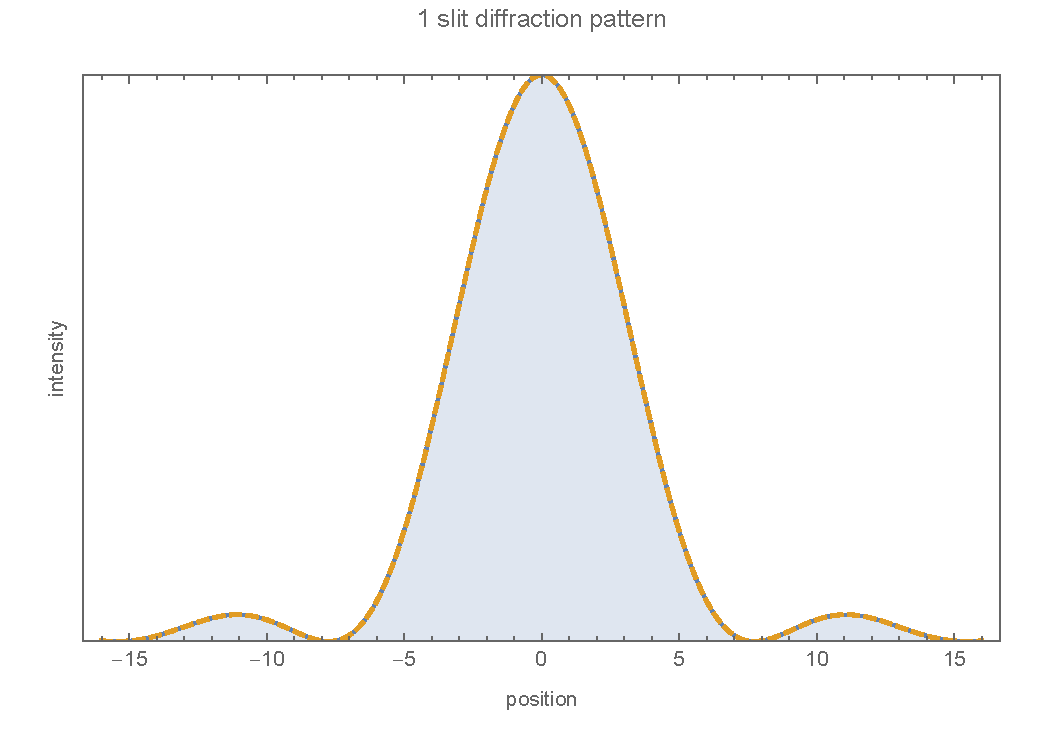
\includegraphics[width=\textwidth]{nslit1}
\end{center}
\column{4cm}
\begin{center}
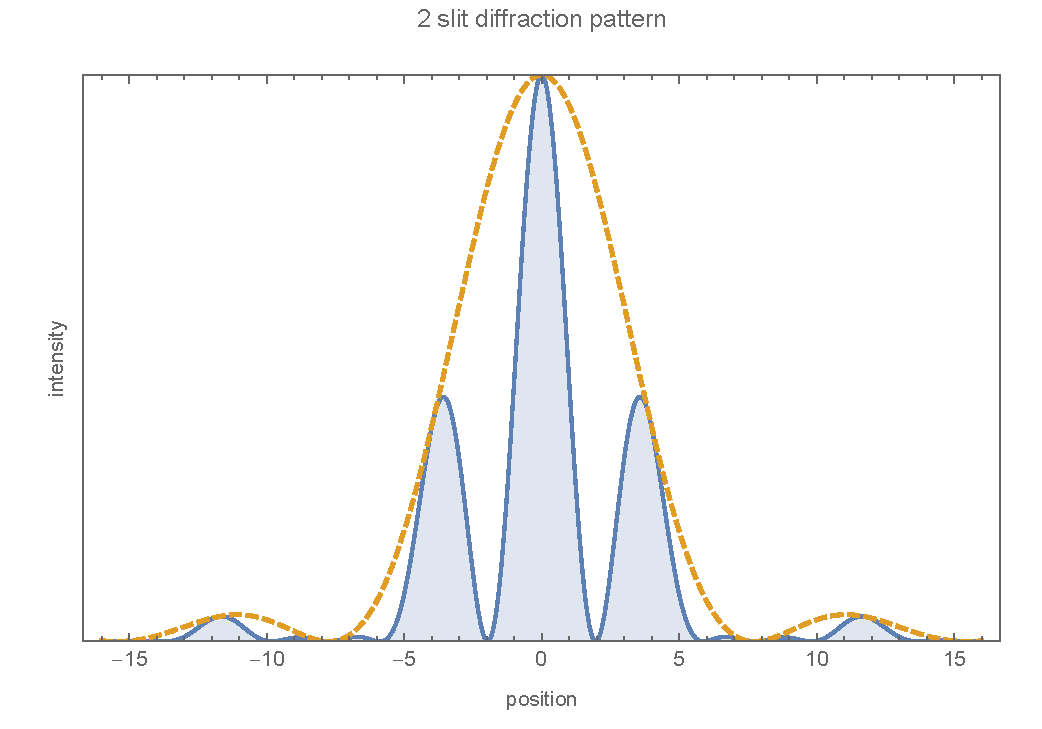
\includegraphics[width=\textwidth]{nslit2}
\end{center}
\column{4cm}
\begin{center}
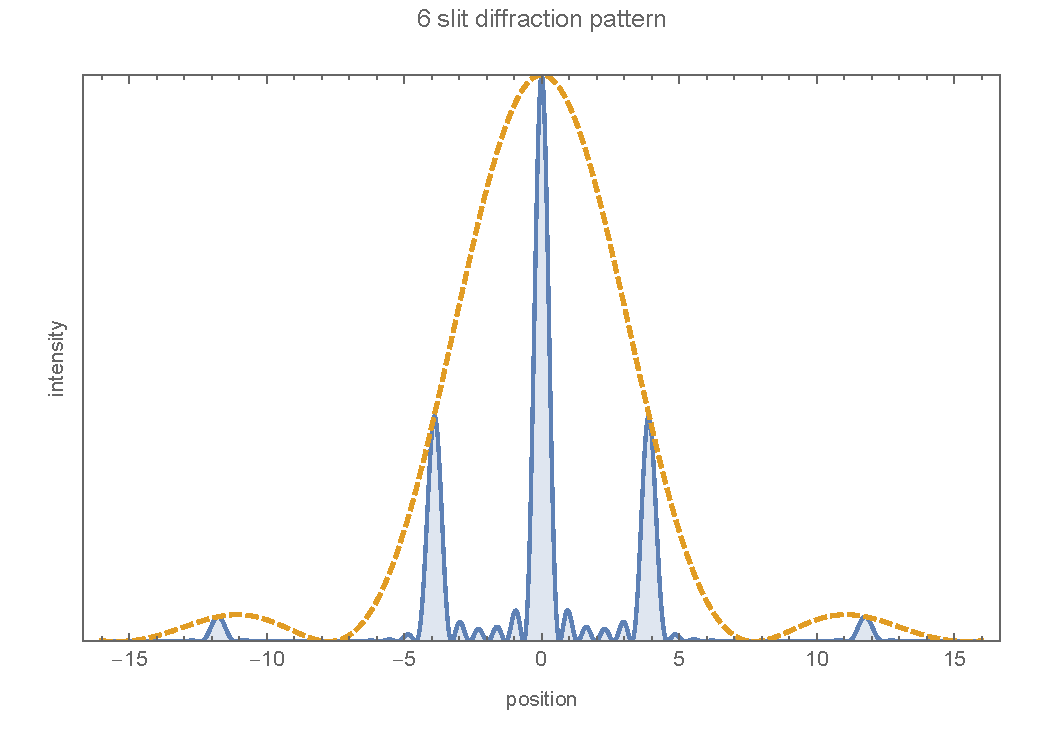
\includegraphics[width=\textwidth]{nslit6}
\end{center}
\end{columns}

Пусть ширина щели $a$, расстояние между щелями $d$, расстояние от маски до экрана $R$, введем нормированный волновой вектор $q=\frac{k\*x}{R}$, где $x$ - текущая координата от центра плоскости изображения. Тогда решение можно получить через полином Чебышева и функцию sinc:

\begin{equation*}
\frac{I}{I_0}=\left[\frac{1}{n}U_{n-1}\left(\cos\left(\frac{d q}{2}\right)\right) \text{sinc}\left(\frac{d a}{2}\right)\right]^2
\end{equation*}
\end{frame}

\begin{frame}{Эффект Тальбо}

\begin{columns}[c]
\column{6.5cm}
\begin{center}
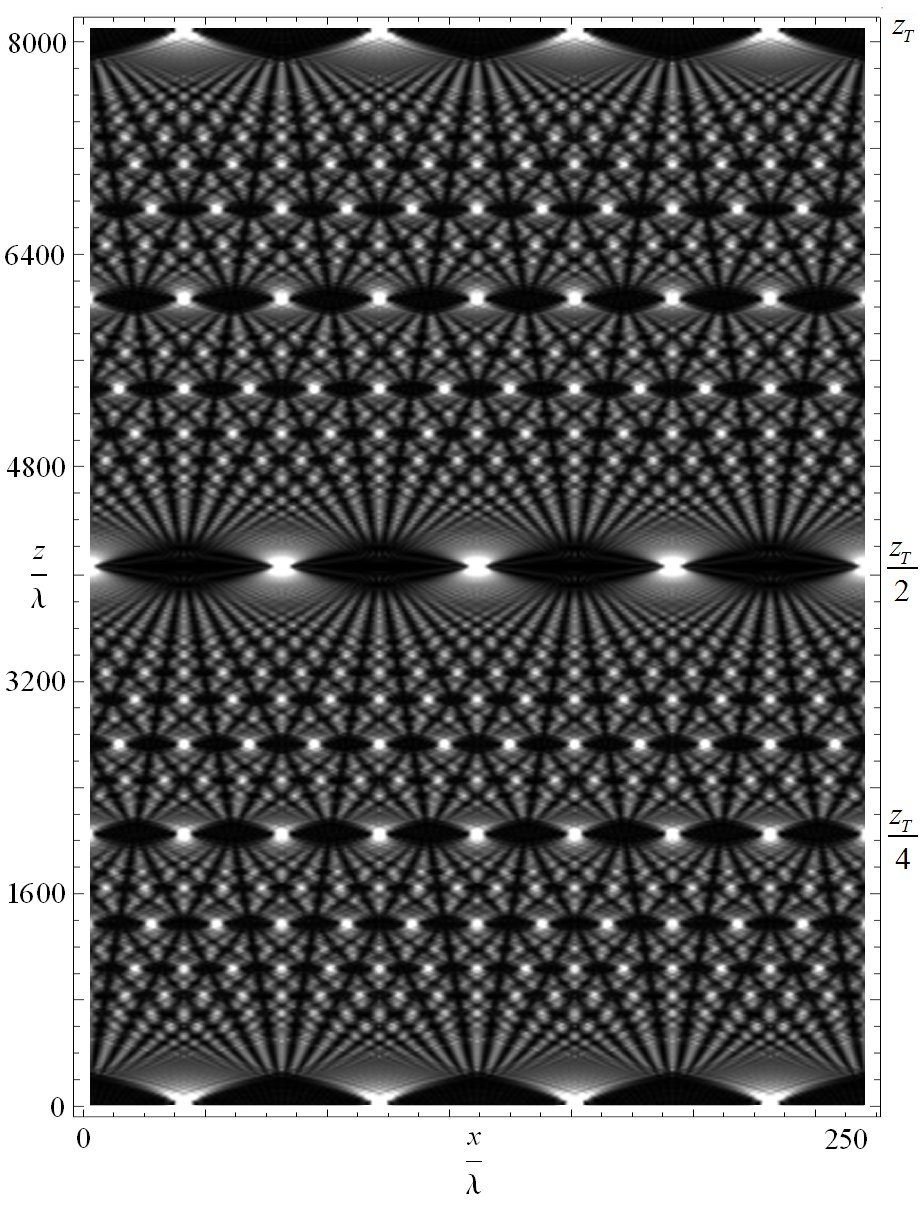
\includegraphics[width=0.9\textwidth]{talbot}
\end{center}
\column{6cm}
\begin{center}
Henry Fox Talbot (1836)

Эффект Тальбо - это характерный для ближней зоны (зоны Френеля) эффект повторения изображения с некоторой характерной длиной, называемой длиной Тальбо

\begin{equation*}
z_T=\frac{2a^2}{\lambda}
\end{equation*}

Уточнение Рэлея
\begin{equation*}
z_T=\frac{\lambda}{1-\sqrt{1-\lambda^2/a^2}}
\end{equation*}
\end{center}
\end{columns}

\end{frame}

\plain{}{Массив щелей как линза}

\begin{frame}{Теоретическое моделирование}
Возбуждение ППП
\begin{columns}[c]
\column{6.5cm}
\begin{center}
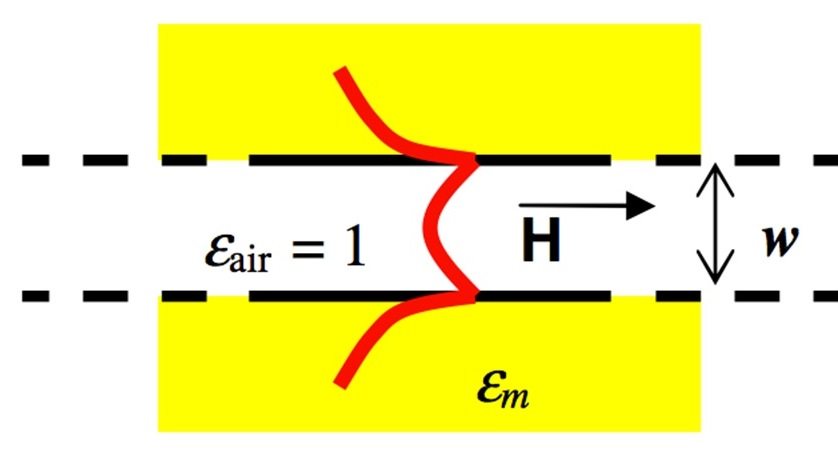
\includegraphics[width=0.9\textwidth]{ns0}
\end{center}
\column{6.5cm}
\begin{center}
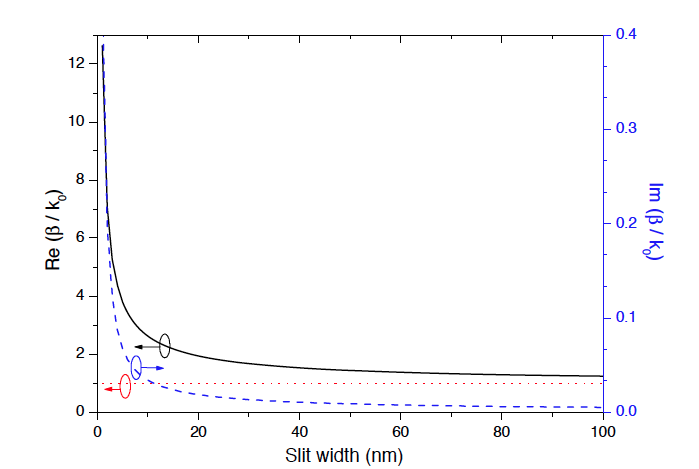
\includegraphics[width=0.8\textwidth]{ns1}

{\tiny для серебра $\epsilon=-17.36+\imath 0.715$ на длине волны 650 нм.}
\end{center}
\end{columns}

\begin{center}
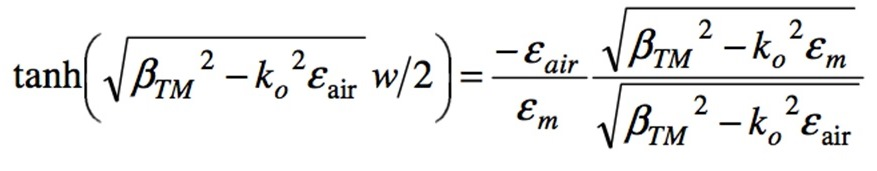
\includegraphics[width=0.7\textwidth]{ns0a}
\end{center}

Когда ширина зазора становится меньше 20 нм, как действительная, так и мнимая часть ВВ плазмона резко возрастает, что указывает на то, что мы достигли условий оптимальных для согласованного распространения двух ППП.

{\tiny Chinese Academy of Sciences, Institute of Optics and Electronics, H.Shi et al. 2005}
\end{frame}

\begin{frame}{Схема эксперимента}
\begin{columns}[c]
\column{6.5cm}
\begin{center}
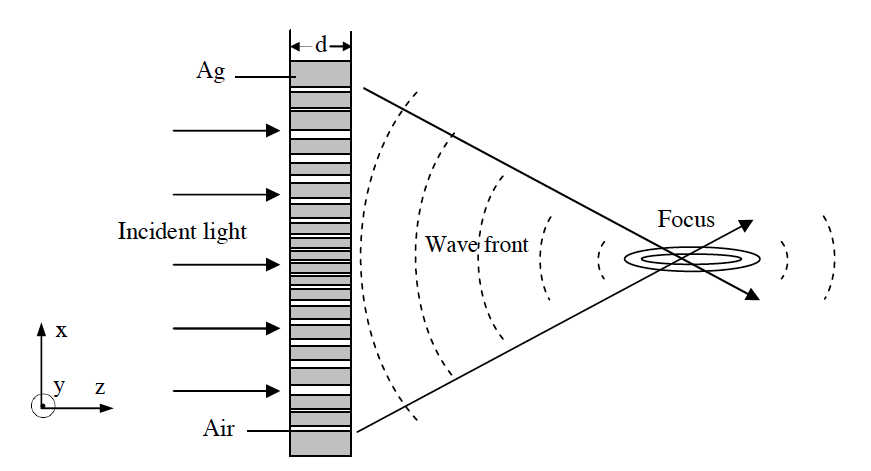
\includegraphics[width=\textwidth]{ns2}
\end{center}
\column{6.5cm}
\begin{center}
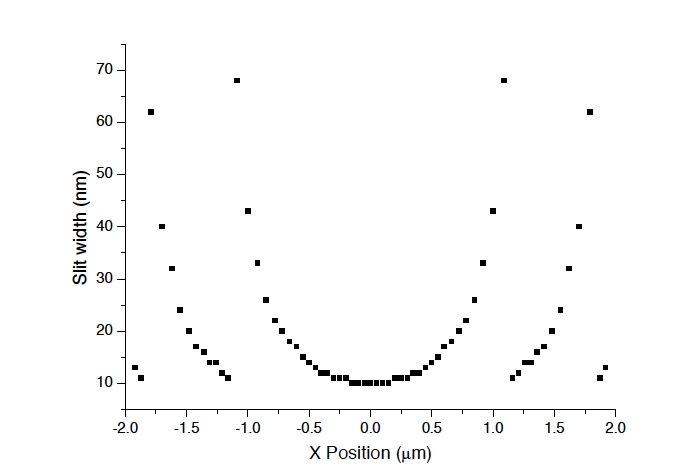
\includegraphics[width=\textwidth]{ns3}
\end{center}
\end{columns}

\begin{equation*}
\phi=\phi_0+\Delta\phi_1+\Delta\phi_2+\beta d+\theta
\end{equation*}

\begin{equation*}
\Delta\phi_1=\text{arg}\left[\frac{n_1-\beta/k_0}{\beta/k_0+n_1}\right]\qquad\Delta\phi_2=\text{arg}\left[\frac{\beta/k_0-n_2}{\beta/k_0+n_2}\right] 
\end{equation*}

\begin{equation*}
\theta=\text{arg}\left[1-\left(\frac{\beta/k_0-n_2}{\beta/k_0+n_2}\right)^2\exp(\imath 2 \beta d)\right] 
\end{equation*}

\end{frame}

\begin{frame}{}

\begin{center}
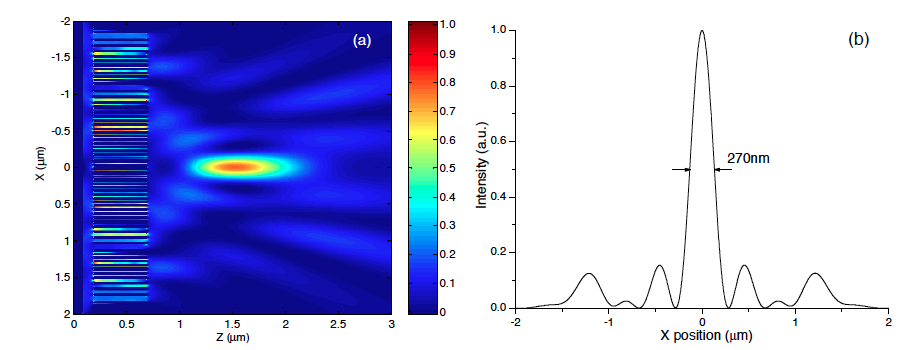
\includegraphics[width=0.9\textwidth]{ns4}
\end{center}

\begin{equation*}
\boxed{\phi(x) = 2n\pi + \frac{2\pi f}{\lambda}-\frac{2\pi\sqrt{f^2+x^2}}{\lambda}}
\end{equation*}

Расстояние между щелями должно быть больше, чем величина скин слоя (для серебра на 650 нм это 24 нм);

Если взять $d=500$ нм, щелевые зазоры меняются в диапазоне от 10 до 70 нм;

Фокусное расстояние такой линзы составило 0.6 микрон;

Пропускающая способность $\approx 60 \%$, при том, что площадь щелей составит треть от общей площади. 

\end{frame}

\begin{frame}{Экспериментальное подтверждение}

Standford Univ., 2009

\begin{columns}[c]
\column{6.5cm}
\begin{center}
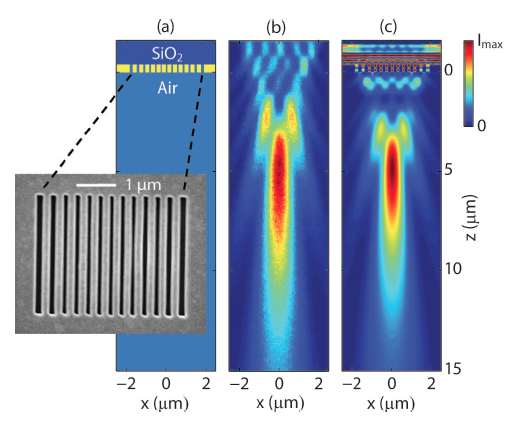
\includegraphics[width=0.9\textwidth]{ns5}
\end{center}
\column{6.5cm}
\begin{center}
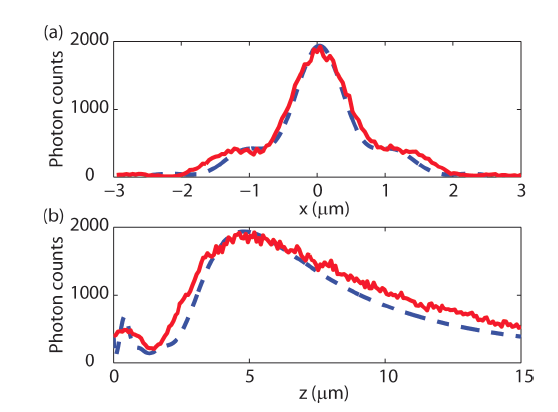
\includegraphics[width=0.9\textwidth]{ns6}
\end{center}
\end{columns}
Видим, что уменьшение количества щелей (от 65 до 12) приводит к заметной делокализации фокального пятна и усложнении его пространственной структуры (боковые лепестки)

\end{frame}


\begin{frame}{Схожая работа на золоте}
\begin{columns}[c]
\column{6.5cm}
\begin{center}
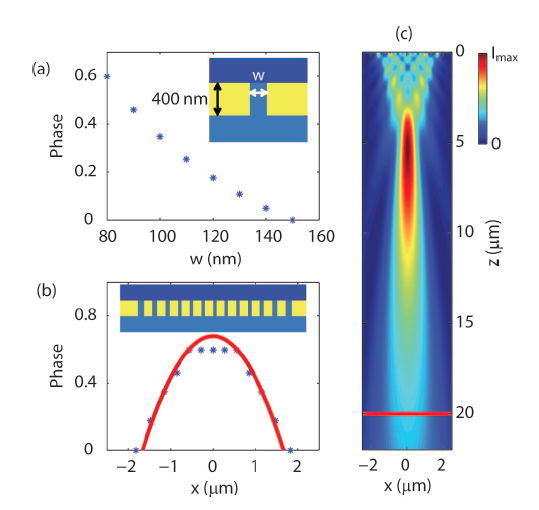
\includegraphics[width=0.9\textwidth]{ns7}

Закон изменения ширины щелей подобран таким образом, чтобы воспроизводить волновой фронт максимально приближенный к цилиндрической волне.

\end{center}
\column{6.5cm}
\begin{center}
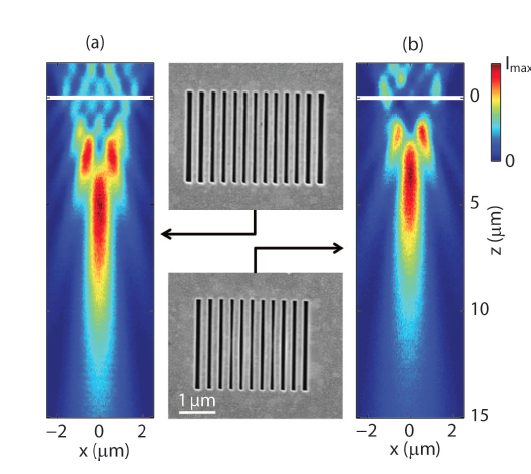
\includegraphics[width=0.9\textwidth]{ns8}

Слева количество щелей 13 (80-150 нм через 2,5 мкм), справа 11 (80-120 нм через 2,5 мкм).

\end{center}
\end{columns}
\end{frame}

\plain{}{Другие виды наноструктурирования}

\begin{frame}{Место в общем ряду методов}
\begin{center}
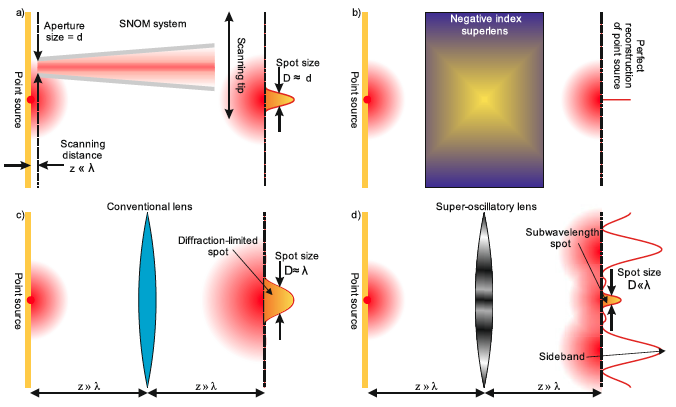
\includegraphics[width=\textwidth]{nh1}
\end{center}

E. Rogers, N. Zheludev. Optical Super-Oscillations: sub-wavelength light focusing and super-resolution imaging. Journal of Optics, 2013
\end{frame}
\begin{frame}{Понятие о сверхосцилляциях}
\begin{center}
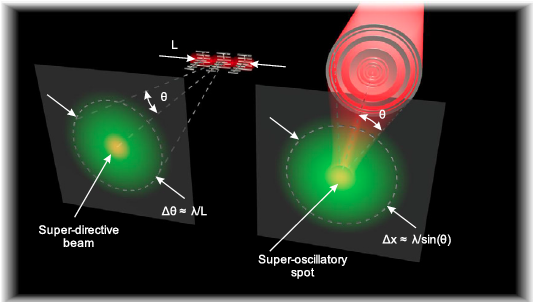
\includegraphics[width=0.8\textwidth]{nh2}
\end{center}

В 1952 году Torraldo di Francia предложил объединить несколько директорных антенн (антенн Яги-Уда) для того, чотбы сделать изображение значительно меньше длины волны. 

Роль массива директорных антенн в оптическом диапазоне играет некоторое предварительно рассчитанное маскирование в поперечной плоскости пучка. Мы теряем в мощности, но пытаемся получить выгоду в разрешении.
\end{frame}

\begin{frame}{Понятие сверхосцилляций}
\begin{columns}[c]
\column{6.5cm}
\begin{center}
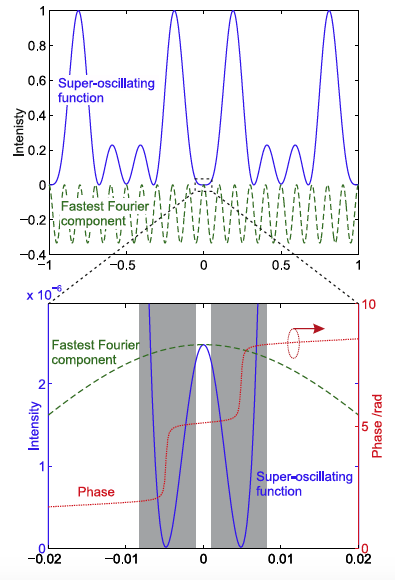
\includegraphics[width=0.9\textwidth]{nh3}
\end{center}
\column{6.5cm}
\begin{center}
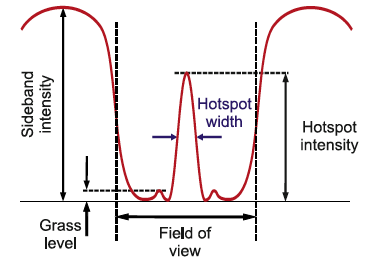
\includegraphics[width=0.9\textwidth]{nh4}

Ааронов показал, что спектрально ограниченная функция может осциллировать быстрее, чем ее самая быстрая фурье-компонента.

Например, $f(x)=(\cos x+\imath \sin x)^N\quad(a>1,N\gg1)$
\end{center}
\end{columns}
\end{frame}

\begin{frame}{Двумерные сверхосцилляции}
\begin{center}
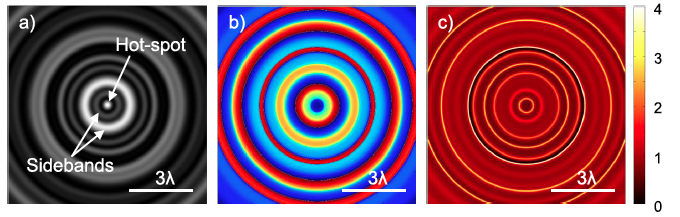
\includegraphics[width=0.9\textwidth]{nh5}
\end{center}

Слева: картина интенсивностей, с т.н. горячим пятном в центре

В центре: соответствующее фазовое распредление, показывающее, что физи в области вокруг горячего пятна очень быстро изменяется

Справа: Величины локальных волновых векторов (области высоокго локального ВВ отвечают СО)

\end{frame}

\begin{frame}{Примеры природных сверхосцилляций}
\begin{center}
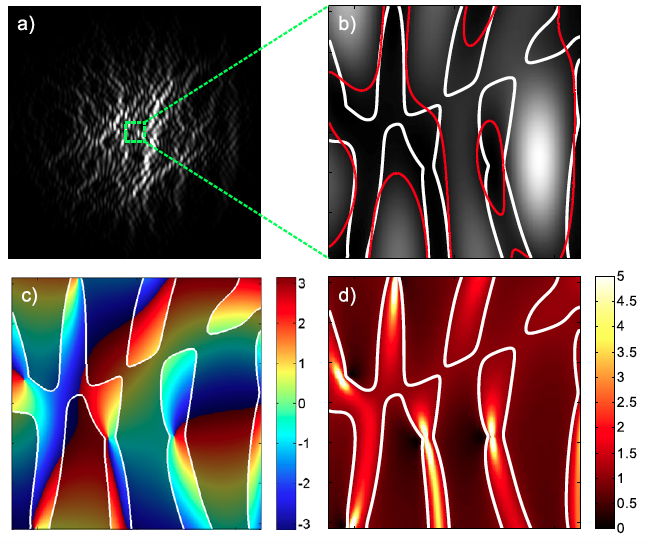
\includegraphics[width=0.7\textwidth]{nh6}

{\small (a) оптические случайные спеклы (получены из интерференции 100 случайно ориентированных плоских волн с одинаковым ВВ), (b) увеличение области сверхосцилляций, (c) фаза в области (b), локальные волновые вектора в масштабе $k_0$}
\end{center}
\end{frame}


\begin{frame}{Конструирование горячего пятна}
\begin{center}
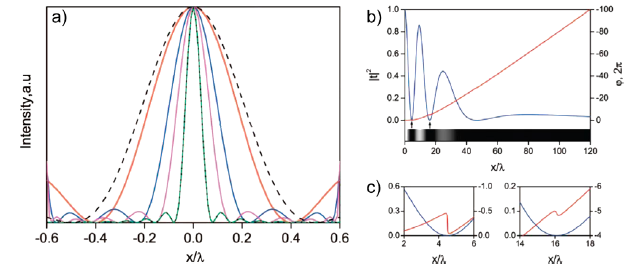
\includegraphics[width=0.9\textwidth]{nh8}
\end{center}
{\small Стартуем с необходимого нам распределения горячего пятна и решаем обратную задачу: какую маску (амплитудную и фазовую) наложить на плоский фронт. 

Если мы ограничиваемся неким пространственным окном, в котором хотим получить горячее пятно, то любая сколь угодно малая особенность поля может быть получена с помощью ряда спектрально-ограниченных функций.

Удобный вариант - эллипсоидальные ВФ, (2-й порядок - красная, 6-й - синяяя, 10-й - розовая, 26-й - зеленая).}
\end{frame}

\begin{frame}{Первое наблюдение, 2007}

При расположении наноотверстий по типу квазикристаллической решетки наблюдались сверхосцилляции.
\begin{center}
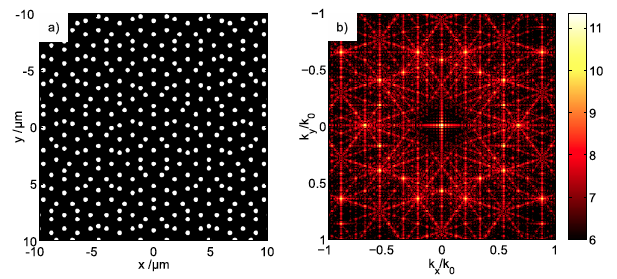
\includegraphics[width=0.65\textwidth]{nh9}

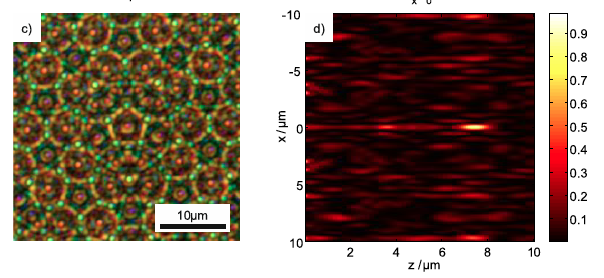
\includegraphics[width=0.65\textwidth]{nh10}

Нижний рисунок справа - ковер Тальбо
\end{center}

\end{frame}

\begin{frame}{Измерение результатов пропускания}
\begin{center}
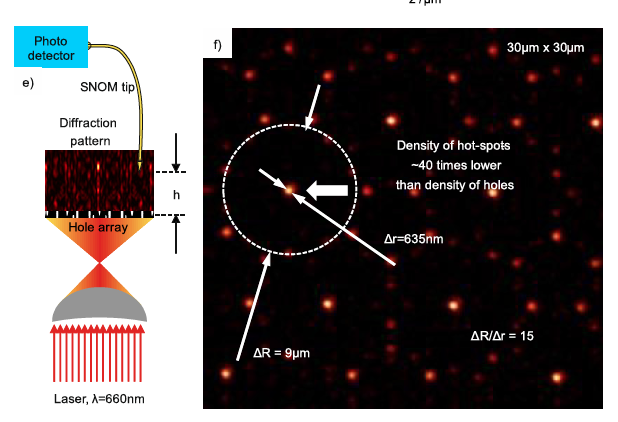
\includegraphics[width=0.8\textwidth]{nh11}

Сохраняется симметрия 5-го порядка. При излучении с длиной волны 660 нм были измерны области размером 235 нм ($\lambda/2 = 330$ нм), что несколько ниже, чем дифракционный предел.
\end{center}

\end{frame}

\begin{frame}{Наноотверстия в квазикристаллическом порядке}
\begin{center}
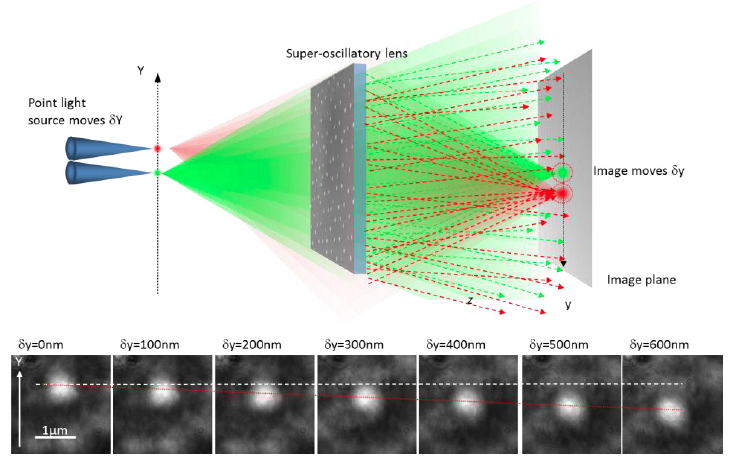
\includegraphics[width=0.8\textwidth]{nh12}
\end{center}
Если использовать кончик  ближнепольного оптического зонда в качестве точечного источника, то можно видеть, что такая структура неискаженно передает сдвиг объекта, сдвиг изображения происходит в обратном направлении на ту же величину
\end{frame}

\begin{frame}{Введение осевой симметрии}
\begin{center}
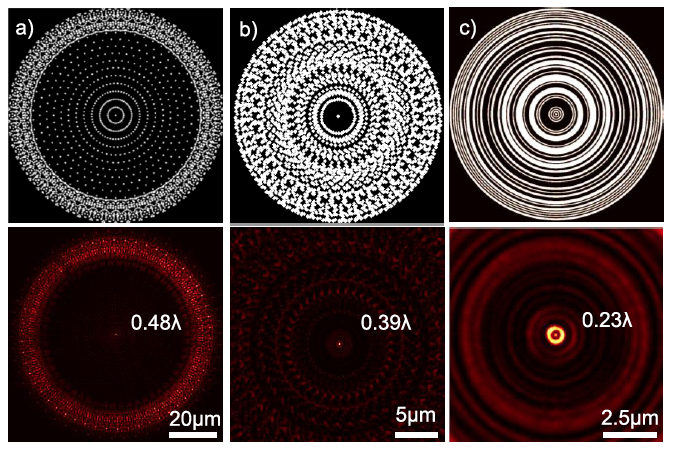
\includegraphics[width=\textwidth]{nh13}
\end{center}
Бинарные маски: (а) 27-й порядок симметрии, (б) - 40-й порядок симметрии (c) - с использованием иммерсионного масла.
\end{frame}

\begin{frame}{Изготовление бинарных масок}
\begin{center}
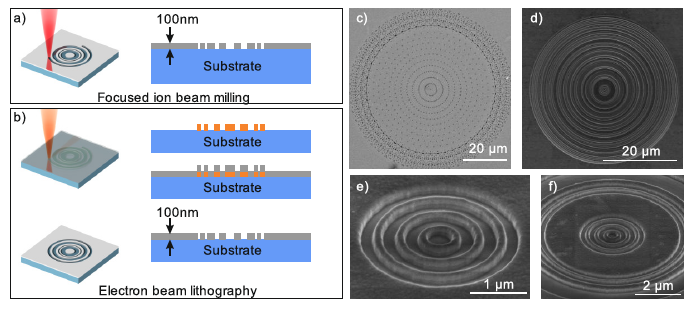
\includegraphics[width=\textwidth]{nh14}
\end{center}

Сверхосцилляционные линзы можно создавать сфокусированным ионным пучком или электроннной литографией.

\end{frame}

\begin{frame}{Изображения на СОЛ}
\begin{center}
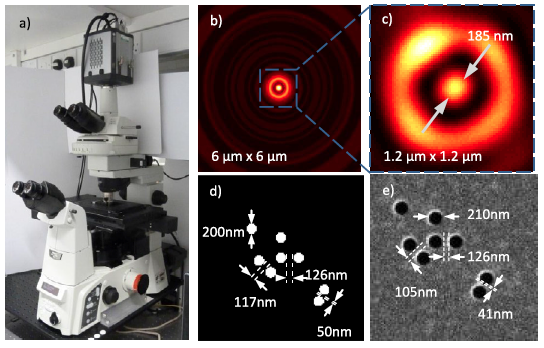
\includegraphics[width=0.9\textwidth]{nh15}

Совмещение СОЛ с традиционным микроскопом с возможностями конфокальных исследований. Получаемое разрешение лучше, чем $\lambda/6$.

\end{center}
\end{frame}


\begin{frame}{Сравнение СОЛ и других методов}
\begin{center}
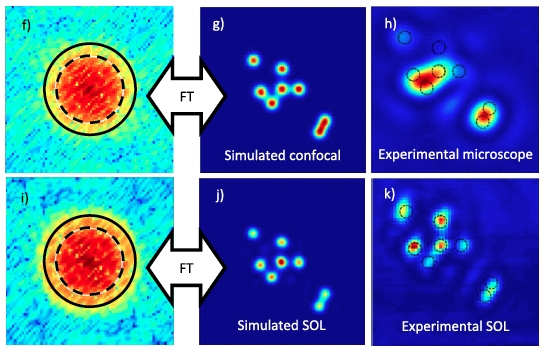
\includegraphics[width=\textwidth]{nh16}
\end{center}

\end{frame}



\plain{}{Теоретическое рассмотрение сверхосцилляций}
\begin{frame}{Эволюция сверхосцилляций}
Эволюция сверхосцилляций: сверхосцилляции исчазают, но значительно медленнее, чем эванесцентные волны

\begin{center}
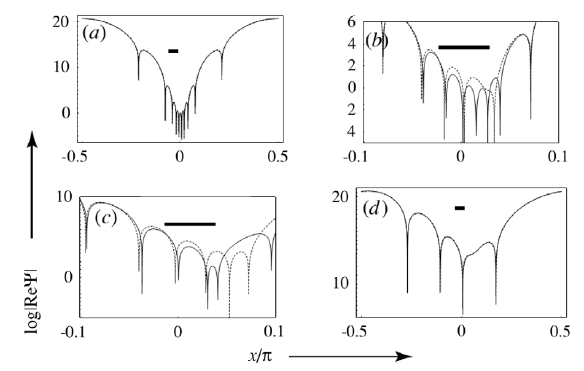
\includegraphics[width=0.8\textwidth]{nh7}
\end{center}

M.V. Berry and S. Popescu. \textbf{Evolution of quantum superoscillations and optical superresolution without evanescent waves}, \underline{Journal of Physics A}. 2006.
\end{frame}

\begin{frame}{Характерные длины}

\begin{equation*}
f(x)=\left(\sin(x)+\imath \cos(x)\right)^N
\end{equation*}

{\small Для случая $a=4$, $N=10$, самая быстрая частота, которая будет присутствовать в фурье-спектре этой функции будет иметь ВВ $2\lambda$.}

Длина, на которой из системы уйдут эванесцентные волны:
\begin{equation*}
z_{evan}\frac{1}{2\sqrt{(aN/d)^2-k^2}}\rightarrow\frac{d}{2aN}<\frac{1}{2k}\approx 0.02
\end{equation*}

Длина, на которой сверхосцилляции дотигнут размера $\lambda$:
\begin{equation*}
z_{\lambda}=\frac{N}{4k}\left(1+\frac{2kd}{aN}+\sqrt{1+\frac{4kd}{aN}-4\left(\frac{kd}{aN}\right)^2}\right)\rightarrow\frac{N}{2k}\approx 0.213
\end{equation*}

Длина, на которой сверхосцилляции достигнут размера $2\lambda$ (т.е. исчезнут)
\begin{equation*}
z_{d}=\frac{kd^2}{4N}\left(1+\frac{2}{a}+\sqrt{1+\frac{4}{a}-\frac{4}{a^2}}\right)\rightarrow\frac{kd^2}{2N}\approx 2.449
\end{equation*}

Длина Тальбо:
\begin{equation*}
z_{T}=\frac{1}{2}\pi k d^2\approx 20 \pi
\end{equation*}

\end{frame}

\begin{frame}{Вспомним историю...}

camera obscura

\begin{center}
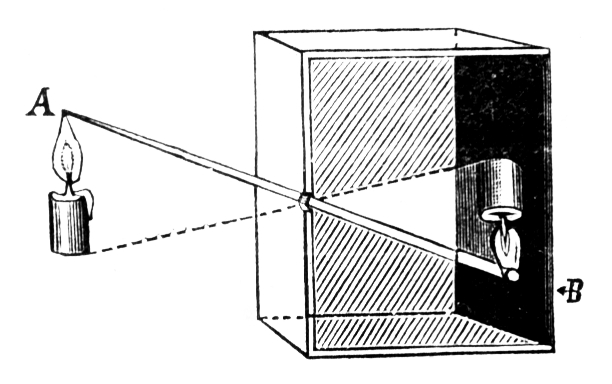
\includegraphics[width=0.8\textwidth]{obscura}
\end{center}



\end{frame}


\end{document}


\begin{frame}{}
\begin{columns}[c]
\column{6.5cm}
\begin{center}
\includegraphics[width=0.9\textwidth]{}
\end{center}
\column{6.5cm}
\begin{center}
\includegraphics[width=0.9\textwidth]{}
\end{center}
\end{columns}
\end{frame}





